In order to make predictions for the NEOCP in the era of LSST, we make simulated observations of a catalogue of solar system objects that takes into account currently known objects. We then use the \dig{} code to calculate NEO scores for each object and use these values to make predictions for the NEOCP. In the subsections below we explain each of these steps in more details.

\subsection{Hybrid Catalogue Pipeline}
Most studies that make predictions for LSST use a synthetic catalogue of solar system objects that doesn't account for prior observations \needcite{}. In reality, we have already detected more than a million objects in the solar system and this number will continue to grow until LSST comes online. This means that, current predictions of detection rates will be inflated since a fraction of ``new'' detections may already be known. Therefore, for this paper we created ``hybrid'' catalogue that combines a synthetic catalogue with all known observations, whilst keeping the population distributions relatively unchanged.

We created the hybrid catalogue to be dynamic, such that we can run a single pipeline to merge in an updated version of \mpco{} as more objects are discovered in the time until LSST comes online. All code to reproduce this hybrid catalogue is open-source and available on GitHub\footnote{\url{https://github.com/dirac-institute/hybrid_sso_catalogue/tree/main/hybridcat/hybridcat}}.

\subsubsection{Data preprocessing}
For the synthetic catalogue of the solar system with we use \sss{}, the Pan-STARRS Synthetic Solar System Model \citep{Grav+2011}. We merge this synthetic catalogue with the latest version of \mpco{}\footnote{\url{https://minorplanetcenter.net//iau/MPCORB.html}}, a database of all currently known objects.

We use \texttt{OpenOrb} \citep{Granvik+2009} to convert both catalogues to Cartesian coordinates and propagate all orbits until the same date.

\subsubsection{Merging algorithm}
The general idea for the merging algorithm is to inject each object from \mpco{} into \sss{}, replacing objects that are similar to those injected. An object's similarity is determined based on its position, $\va{x}$, velocity, $\va{v}$, and absolute magnitude (size), ${H}$.

We split each catalogue into bins of absolute magnitude linearly spaced from $-2$ to $28$ and perform the merge algorithm on each bin separately. For each bin we build a K-D trees for both catalogues based on the positions ($x, y, z$) of objects. For every MPCORB object we query the S3M tree for the nearest $100$ objects up to a maximum distance of $0.1 \unit{AU}$, excluding any that have already been matched to a different real object. From these remaining nearest neighbours, we select the S3M object with the closest velocity as the matched object. If there were no remaining neighbours, either because no synthetic objects were nearby or because all nearby objects had already been matched, then we directly add this real object without replacing a synthetic one.

To complete the merging process, we compile the matched object IDs and delete them from S3M. We then add the entirety of MPCORB to the remaining catalogue, resulting in a hybrid catalogue.

\subsubsection{Assessing quality of hybrid catalogue}
It is essential that the underlying distributions of the hybrid catalogue do not differ significantly from S3M so that we still accurately reproduce the solar system. In Figure~\ref{fig:hybrid_vs_s3m_dists}, we show the distributions of the absolute magnitude and six orbital elements in both the hybrid catalogue and S3M. It is evident that the distributions are essentially identical.

\begin{figure*}[htb]
    \centering
    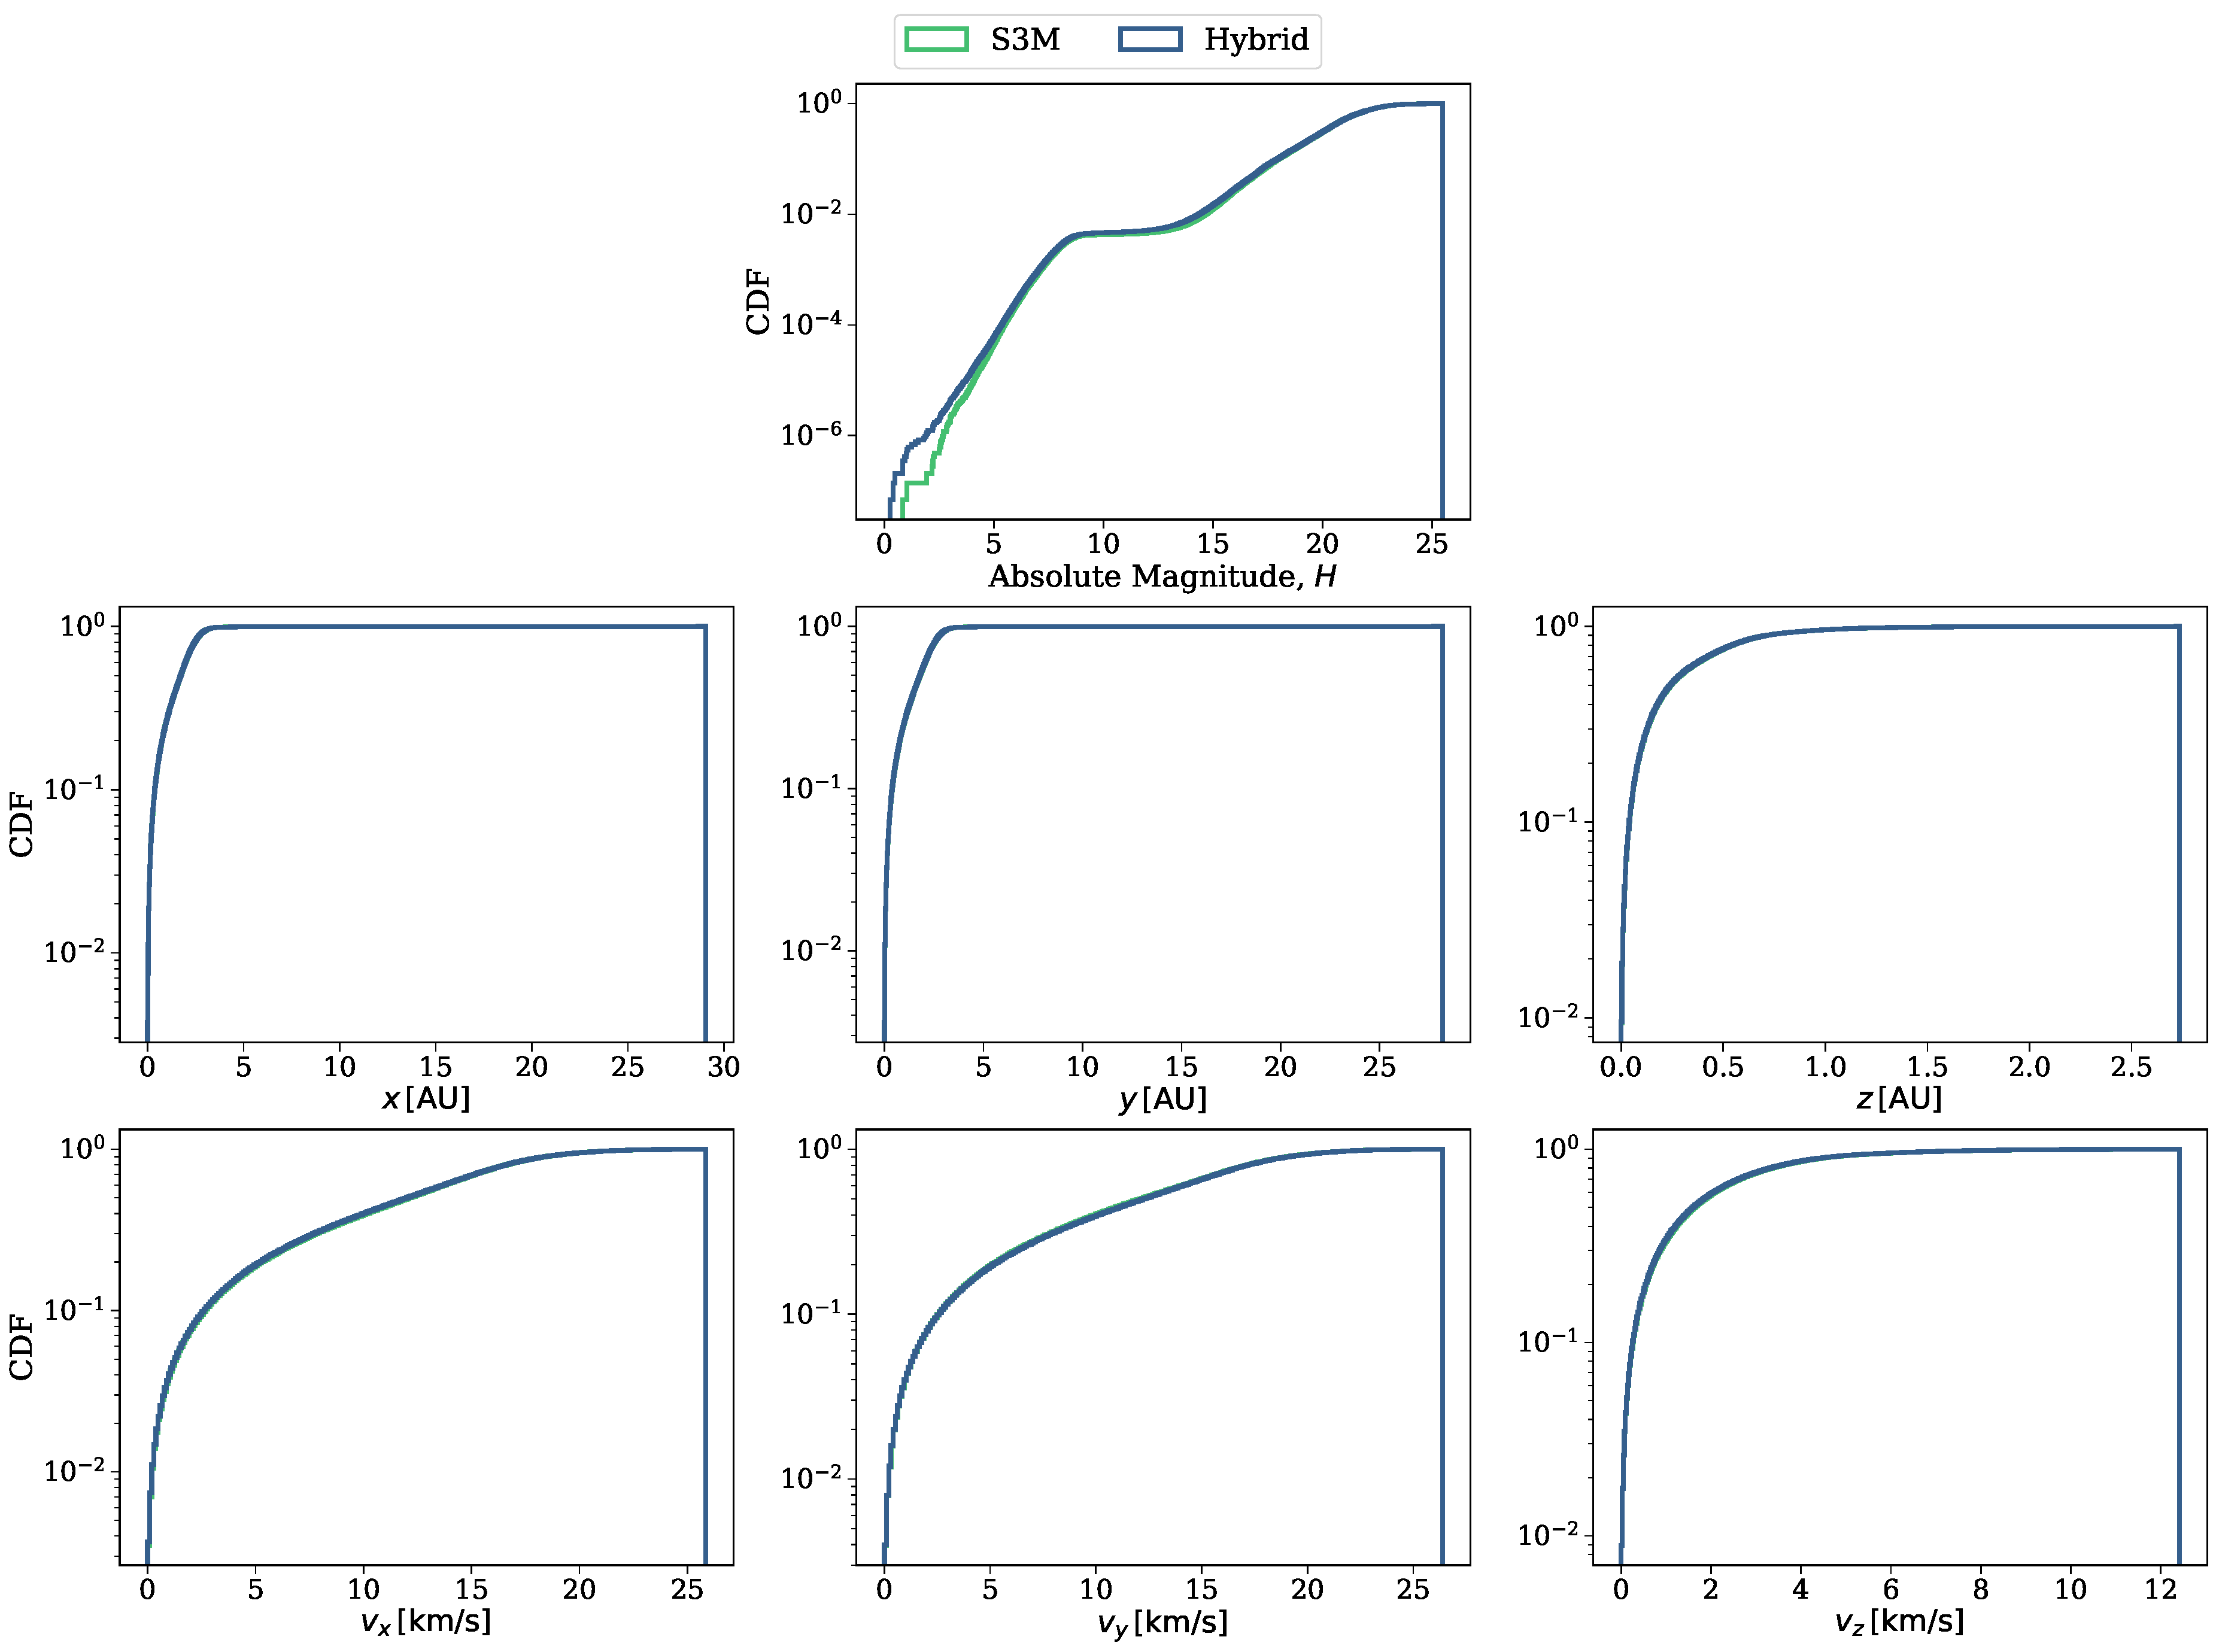
\includegraphics[width=\textwidth]{hybrid_vs_s3m_distributions.pdf}
    \caption{A comparison of the parameter distributions of S3M and the hybrid catalogue.}
    \label{fig:hybrid_vs_s3m_dists}
\end{figure*}

As a further check, we compared MPCORB to the objects that were removed from S3M, since these should have nearly identical distributions. In Figure~\ref{fig:density_compare}, we show a comparison of the densities for the heliocentric $x$ and $y$ and it is clear that these distributions are left unchanged in the hybrid catalogue.

\begin{figure}[htb]
    \centering
    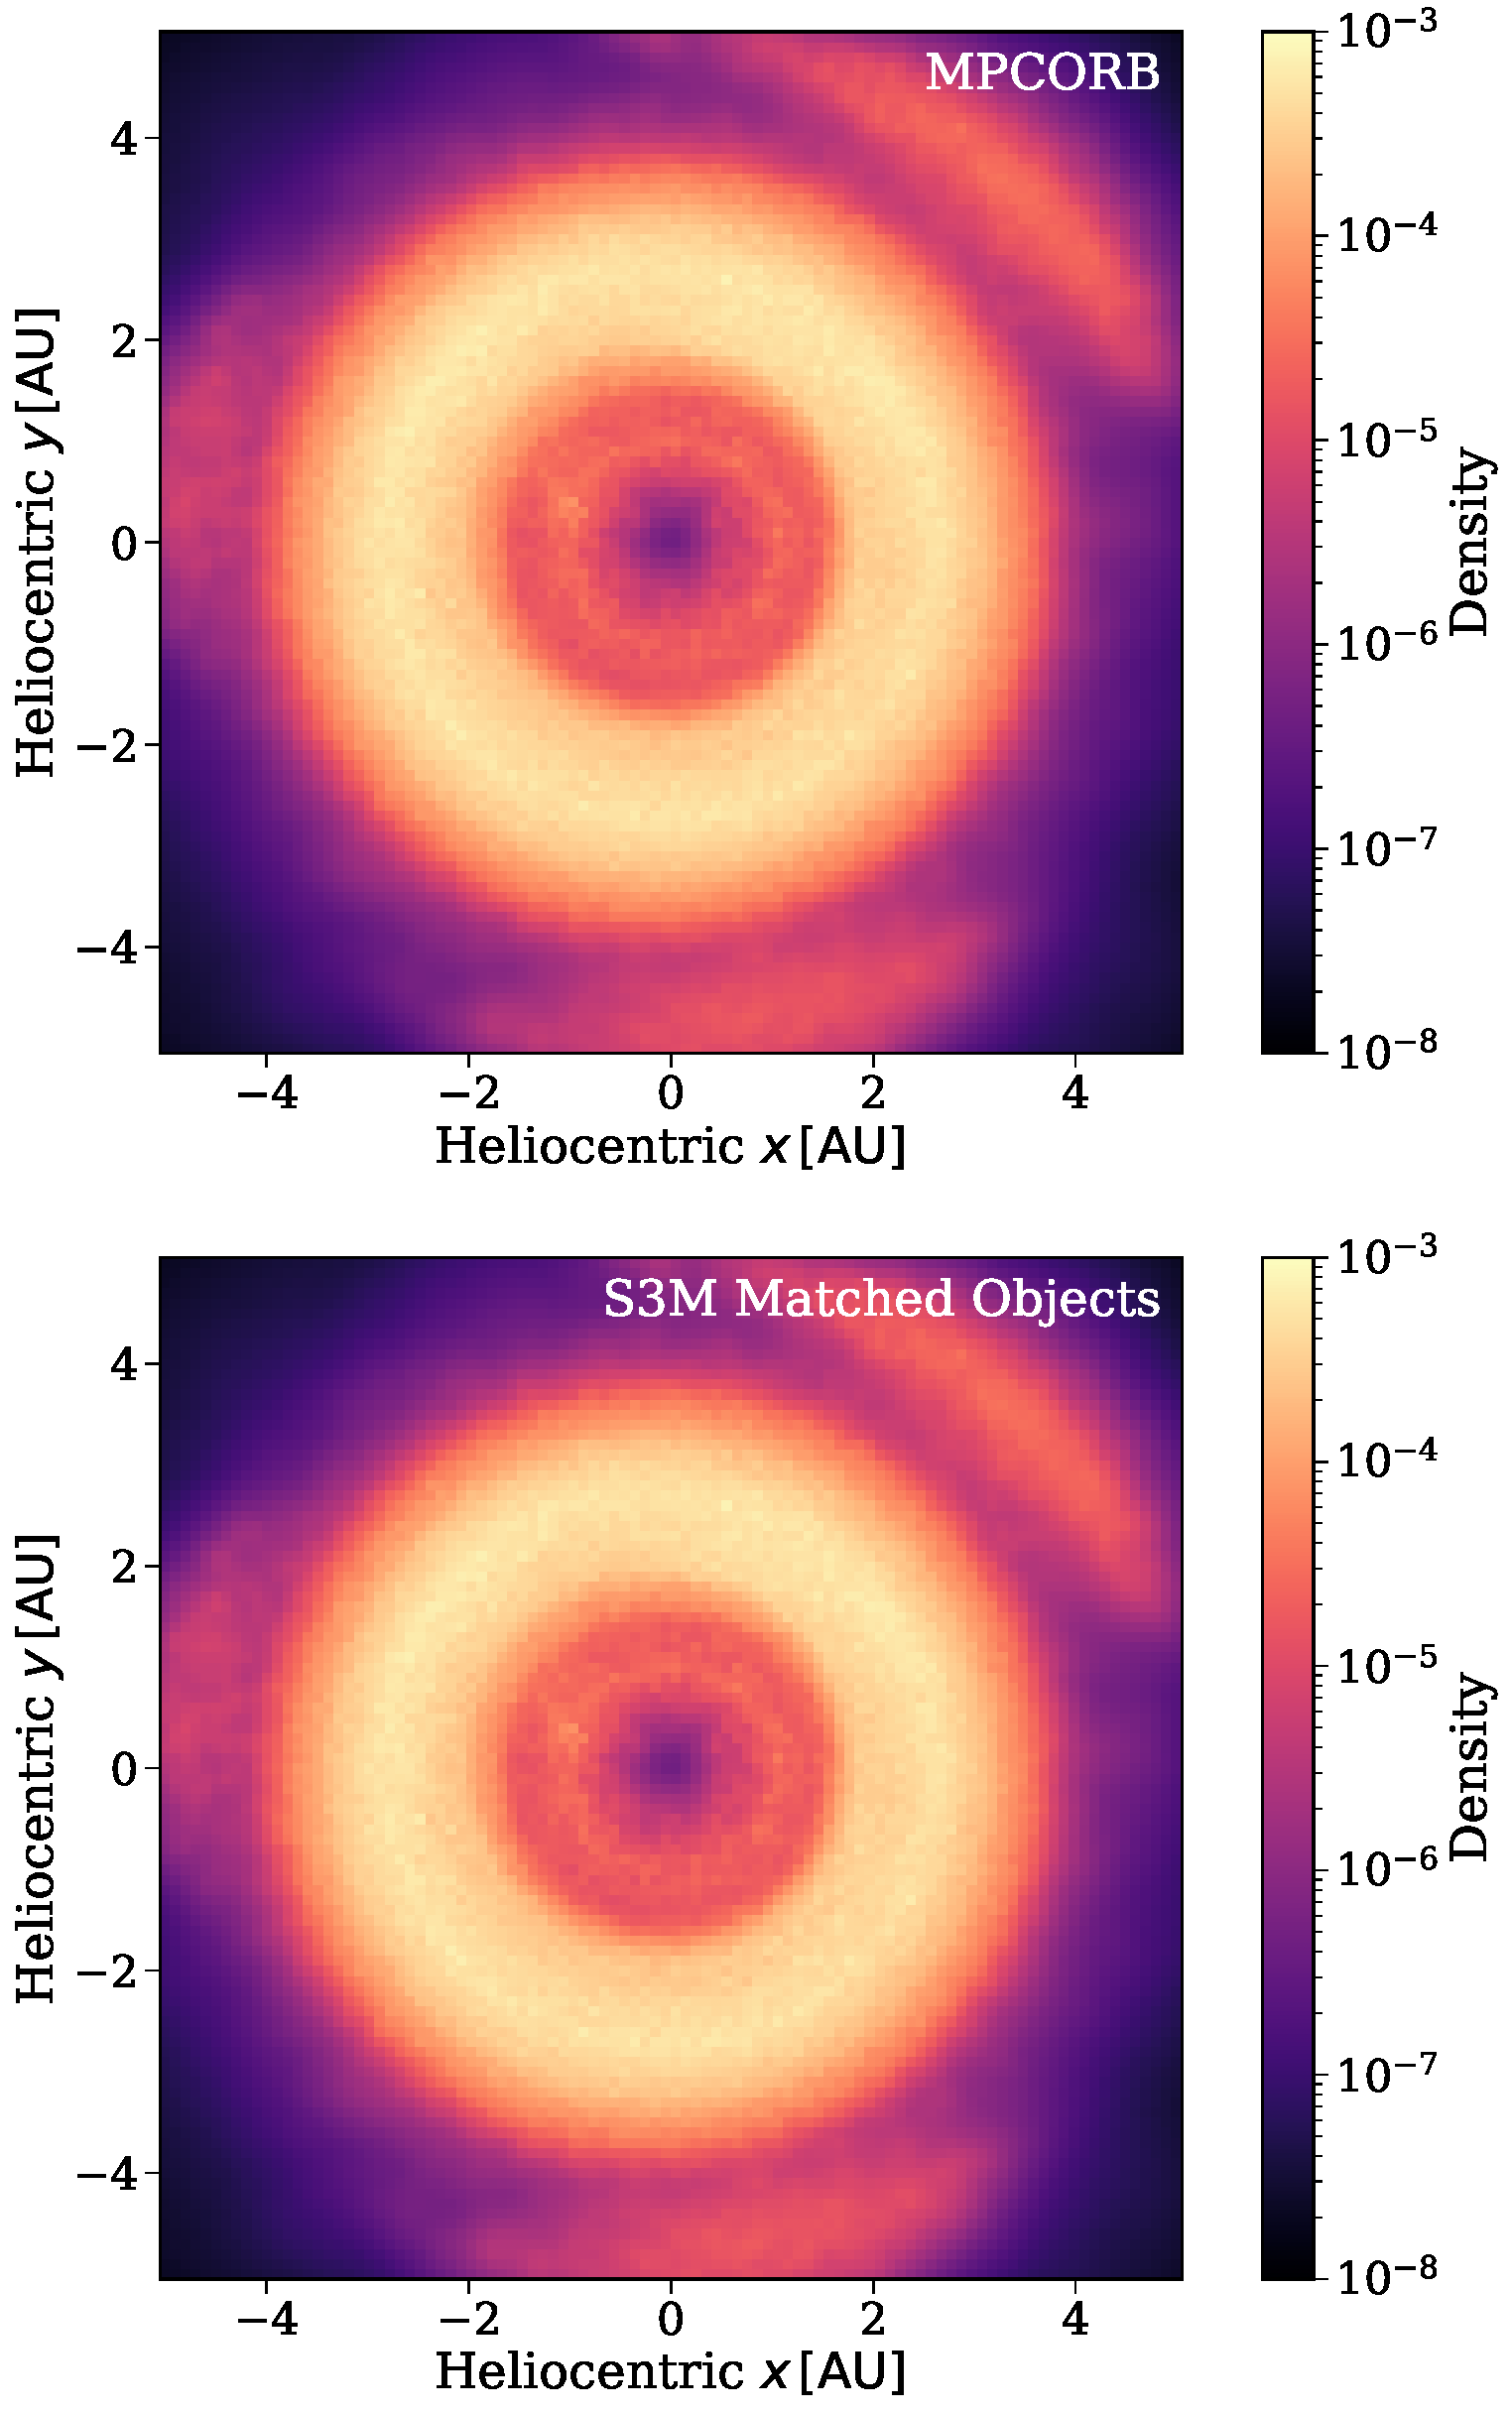
\includegraphics[width=\columnwidth]{density_comparisons.pdf}
    \caption{A comparison of the density of \mpco{} objects with those objects that were matched in \sss{} by our hybrid catalogue pipeline.}
    \label{fig:density_compare}
\end{figure}

\begin{figure}[htb]
    \centering
    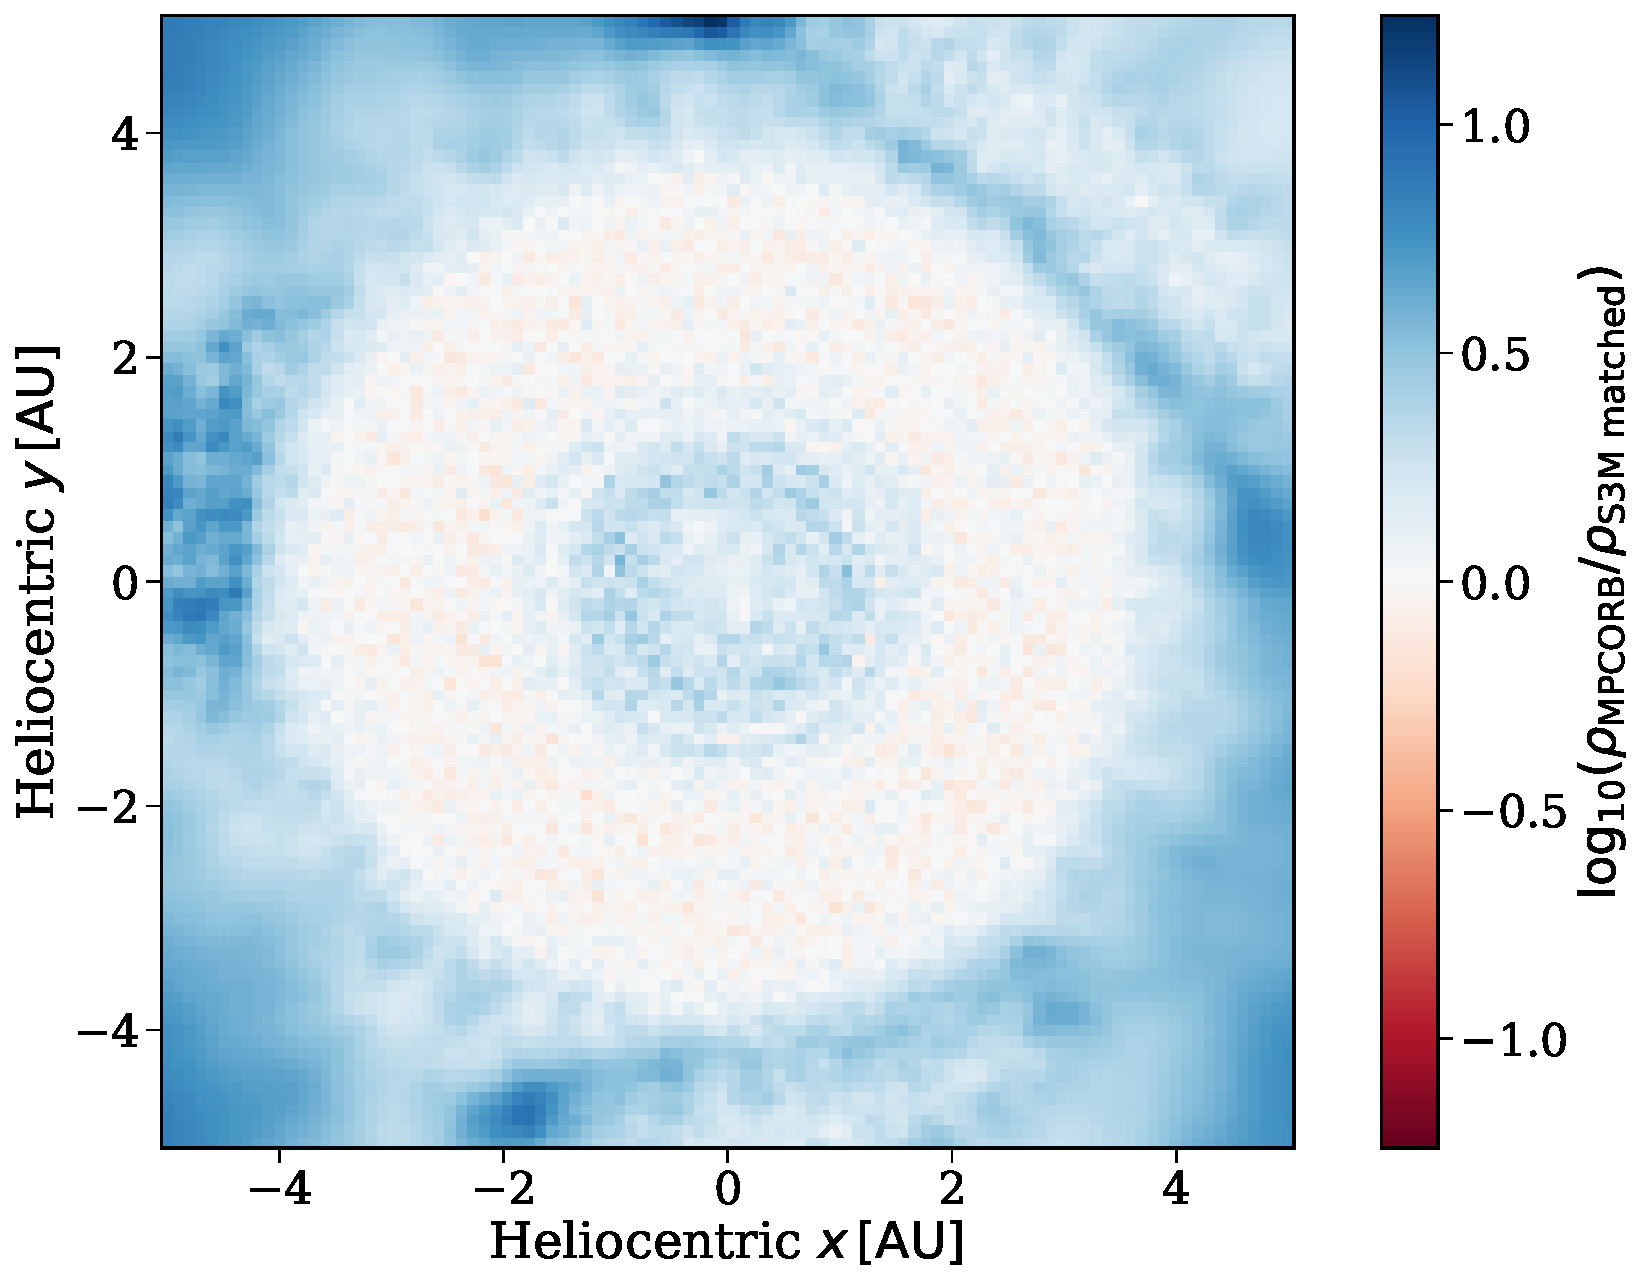
\includegraphics[width=\columnwidth]{density_residuals.pdf}
    \caption{}
    \label{fig:density_residuals}
\end{figure}

\subsection{Simulated Observations}

\todo{Should probably talk about whatever Sam did here \needcite{}}

\subsection{\dig{} Score Calculation}
\subsubsection{Tracklet submission cuts}


\subsection{LSST Discovery probability}
\todo{}
